\chapter{Best Things about MTJs}


\section{Critical Voltage Measurement}




\section{Field Modulated Mag-noise Measurement}



The UCI group developed a novel method of experimental characterization of the spectrum of spin wave eigenmodes of individual STT-MRAM elements. This method is magnetic noise spectroscopy with magnetic field modulation. Figure 3(a) shows the experimental setup for measuring magnetic noise with magnetic field modulation, in which a microwave-frequency noise emitted by the STT-MRAM at a finite bias current is measured via a lock-in detection

\begin{figure}[!ht]
  \centering
  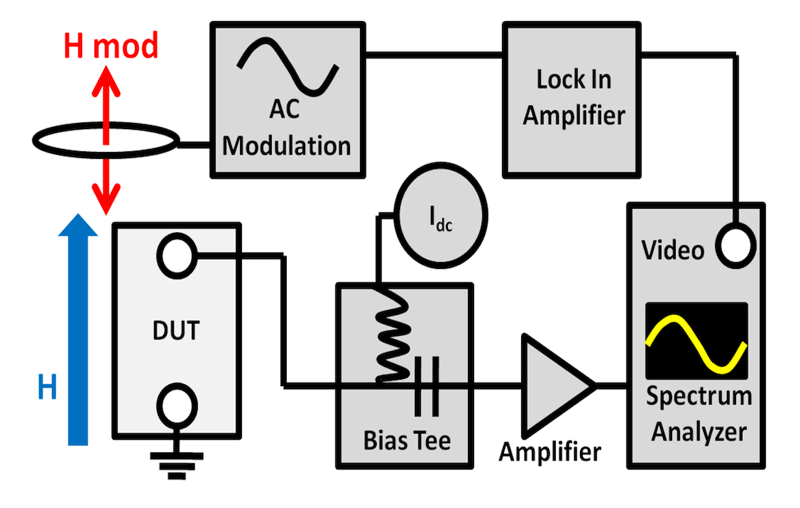
\includegraphics[width=0.6\textwidth]{fig/magnoise/Picture1.png}
   \caption{Set-up for Magnoise measurement}
  \label{fig:magnoise-setup}
\end{figure}

technique. The microwave noise is emitted at the frequencies of spin wave eigenmodes of the sample, with the most prominent features arising from spin wave eigenmodes of the free layer. The top panel of Figure 3(b) shows the magnetic noise spectrum measured by conventional technique without magnetic field modulation. The conventional method only allows us to reliably measure the frequency of the quasi-uniform spin wave mode. 






In contrast, the data obtained with magnetic field modulation shown below allow us to detect not only the resonant frequencies but also the spectral linewidth of several spin wave modes of the device. This is enabled by the superior signal-to-noise factor of our technique with magnetic field modulation. The data obtained with magnetic field modulation is of high enough quality to enable determination of the Gilbert damping, magnetic anisotropy and exchange stiffness constant of the free layer. The main feature of the magnetic noise method is that it allows measurement of the spin wave spectrum faster than the ST-FMR method.  Therefore, this method can be used for rapid screening of magneto-dynamic properties of STT-MRAM cells.




\begin{figure}[!ht]
  \centering
  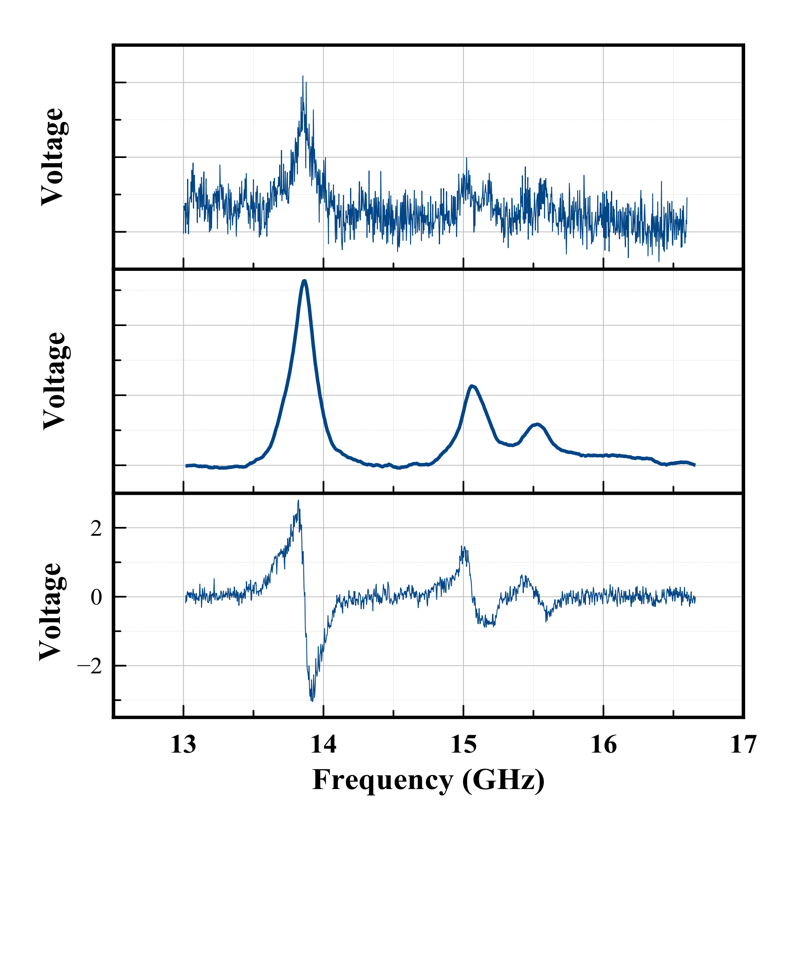
\includegraphics[width=0.6\textwidth]{fig/magnoise/magnoise-data.png}
   \caption{Set-up for Magnoise measurement}
  \label{fig:magnoisedata}
\end{figure}


\begin{figure}[!ht]
\centering
\subfigure{\label{fig:noiseMR}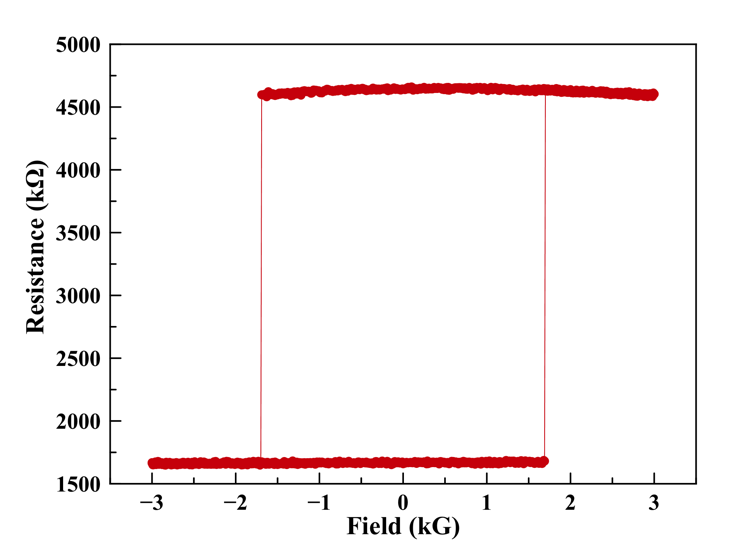
\includegraphics[width=75mm]{fig/magnoise/noiseMR}}
\subfigure{\label{fig:noiseFMR2D}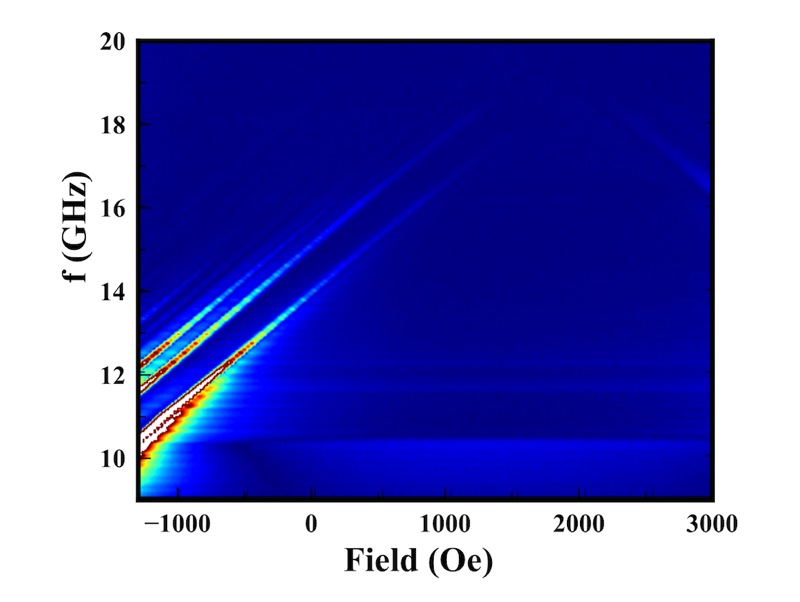
\includegraphics[width=75mm]{fig/magnoise/noiseFMR2D}}
\caption{(a) AP state simulation (b)P state simulations}
\end{figure}



\begin{figure}[!ht]
  \centering
  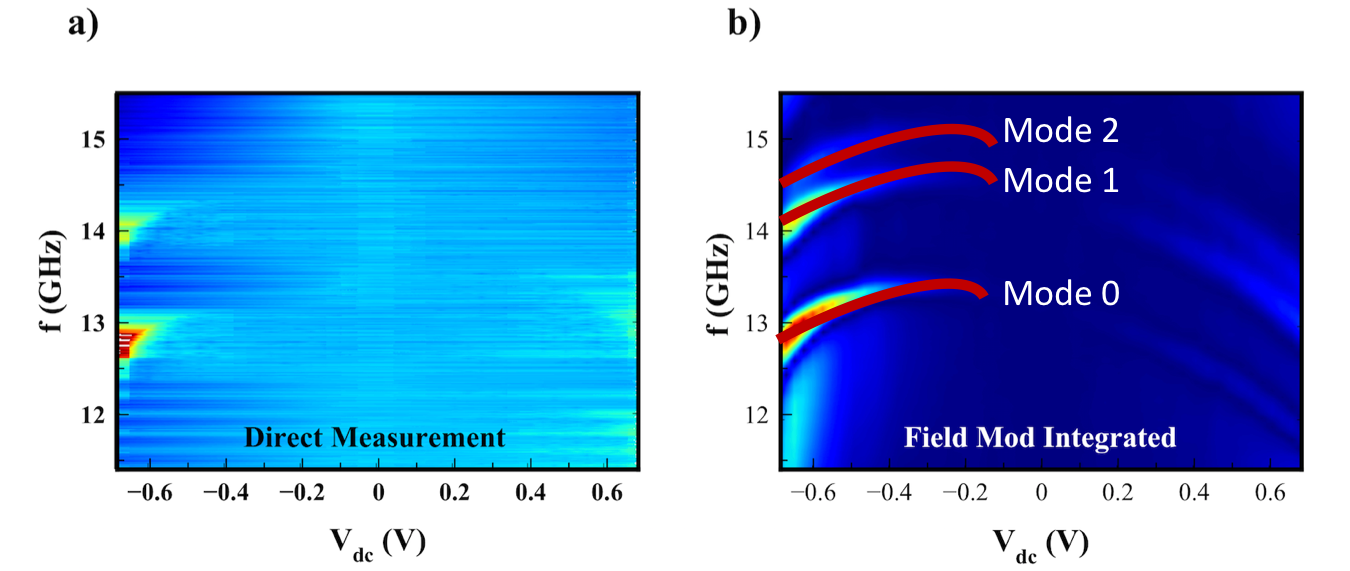
\includegraphics[width=1.0\textwidth]{fig/magnoise/magnoise2D.png}
   \caption{Set-up for Magnoise measurement}
  \label{fig:magnoise-2D}
\end{figure}



\begin{figure}[!ht]
\centering
\subfigure{\label{fig:FMRfreq}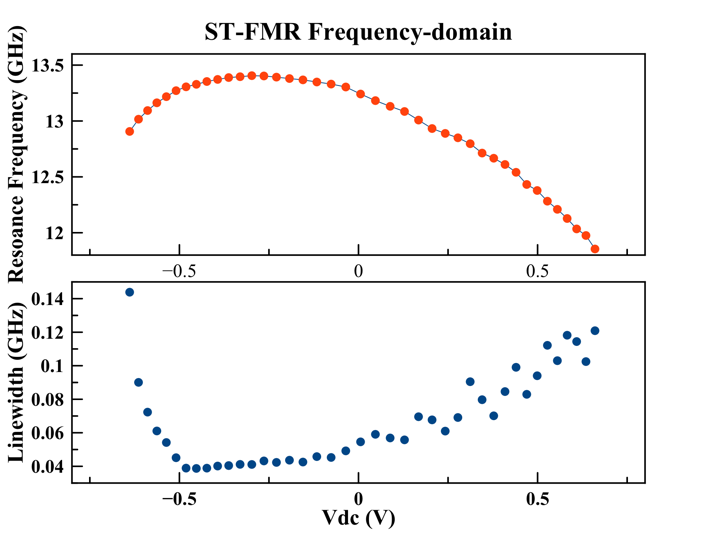
\includegraphics[width=75mm]{fig/magnoise/STFMR-freq.png}}
\subfigure{\label{fig:Noisefreq}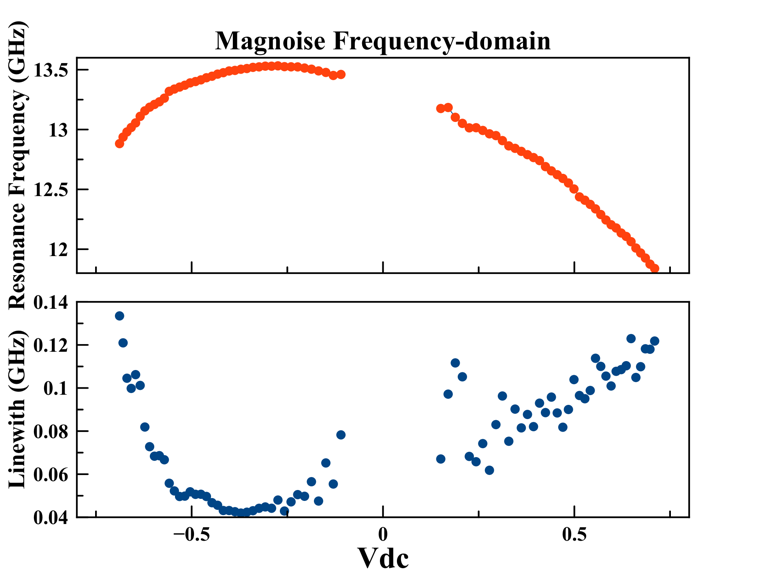
\includegraphics[width=75mm]{fig/magnoise/noise-freq}}
\caption{(a) ST-FMR data on the frequency domain (b) Magnoise data on the frequency domain}
\end{figure}




\begin{figure}[!ht]
\centering
\subfigure{\label{fig:FMRfield}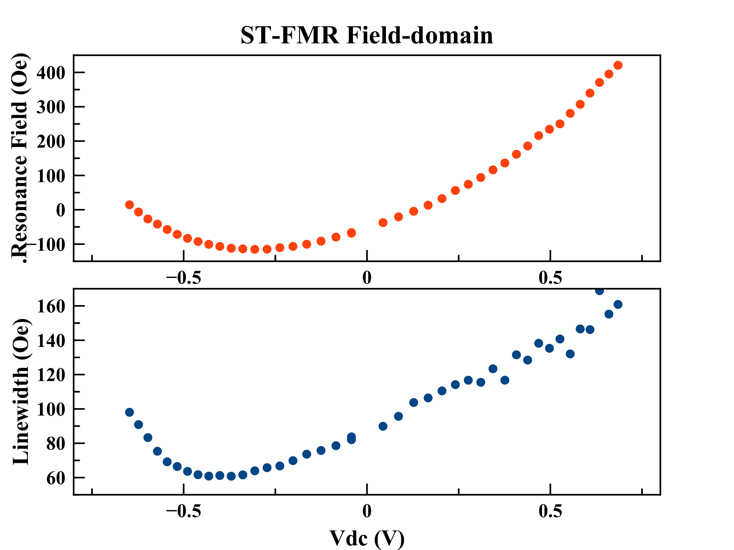
\includegraphics[width=75mm]{fig/magnoise/FMR-field}}
\subfigure{\label{fig:Noisefield}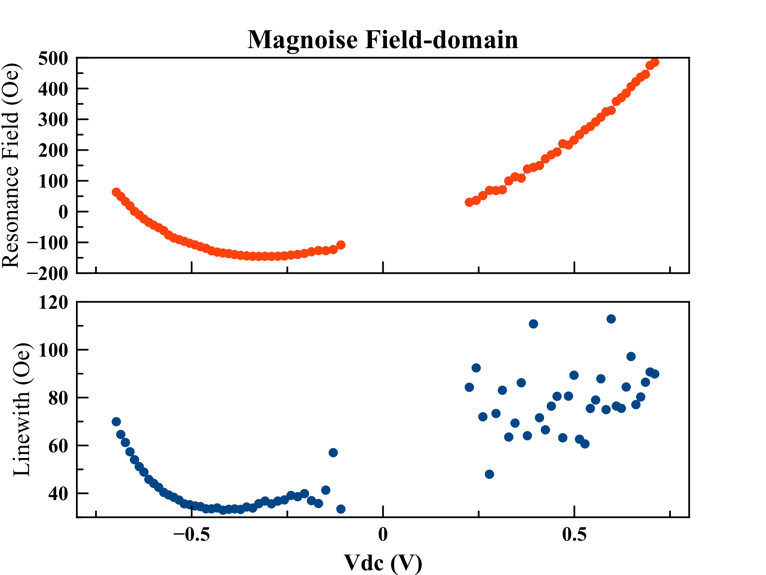
\includegraphics[width=75mm]{fig/magnoise/noise-field}}
\caption{(a) ST-FMR data on the field domain (b) Magnoise data on the field domain}
\end{figure}






\clearpage

\section{In-plane ST-FMR measurement and Mode identification}

While the Spin-torque Ferromagnetic Resonance(ST-FMR) technique is a powerful tool of detecting the spin-wave eigenmodes within the free layer of the Magnetic Tunnel Junctions(MTJs), one needs to be careful about the "modes" excited in the experimental spectrum. There are two main concerns here. First of all, it is important to excite all the spin wave modes of the free layer, from the lowest-frequency quasi-uniform mode to higher modes. Due to different excitation mechanism, either the quasi-uniform mode or some of the higher order modes are possible to be weak in the ST-FMR signal. Mislabelling the modes makes further analysis impossible. 
 Furthermore, as we have seen from the previous chapter, exchange coupling between the free layer and the SAF layer, if not dominant, does exist within the MTJs. Most of the time, we are mainly interested in the free layer dynamic properties and we do not wish to have SAF layer modes mixed with the free layer modes. These two problems are better explained in the following example.

\begin{figure}[!ht]
\centering
\subfigure{\label{fig:S6AP}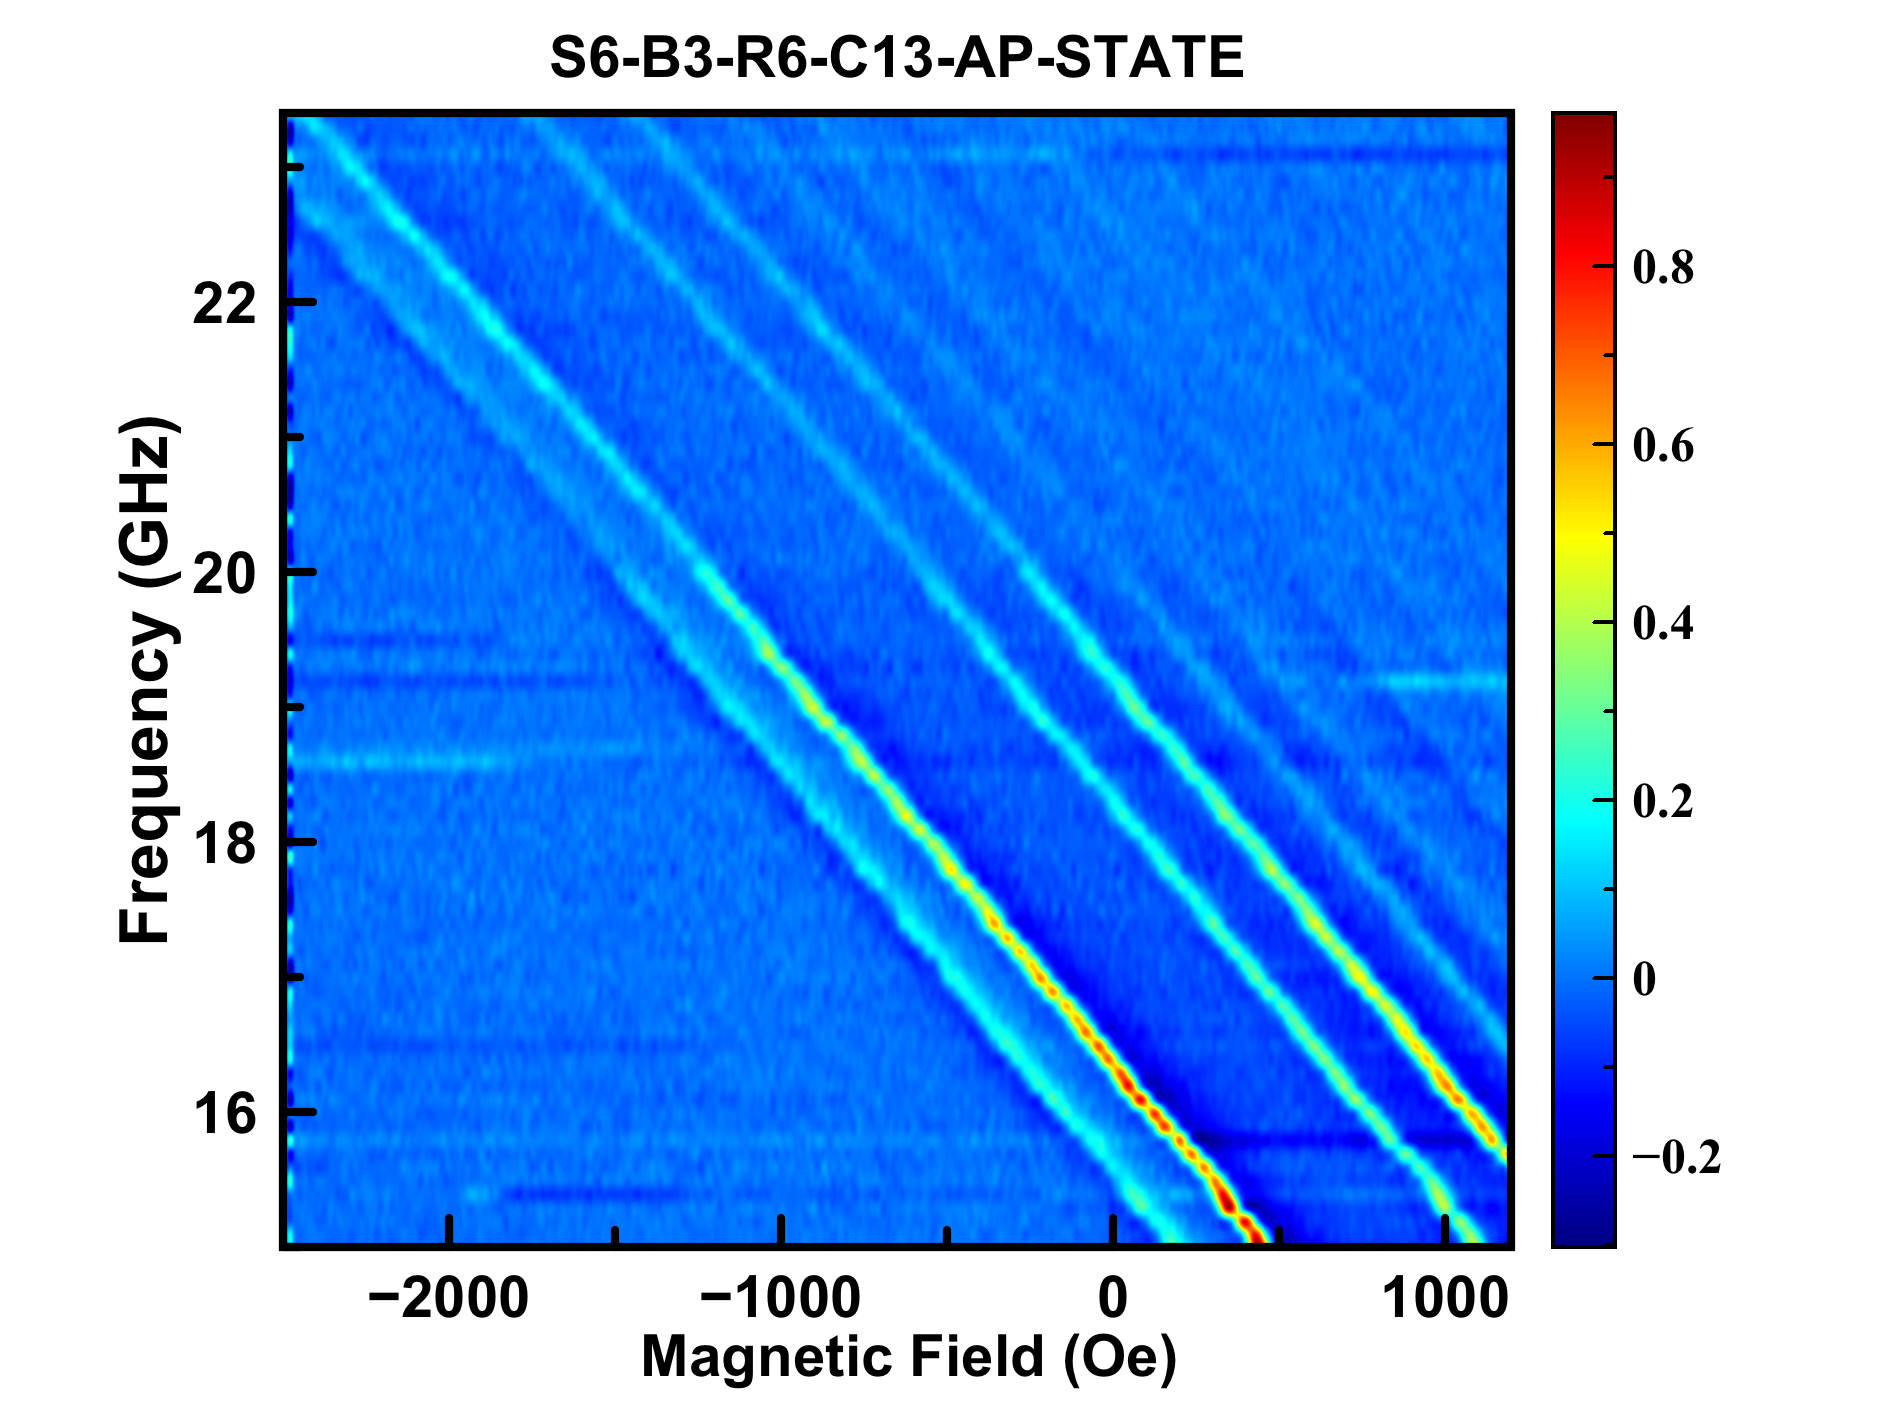
\includegraphics[width=75mm]{fig/in-plane/S6-B3-R6-C13-AP-STATE}}
\subfigure{\label{fig:S6P}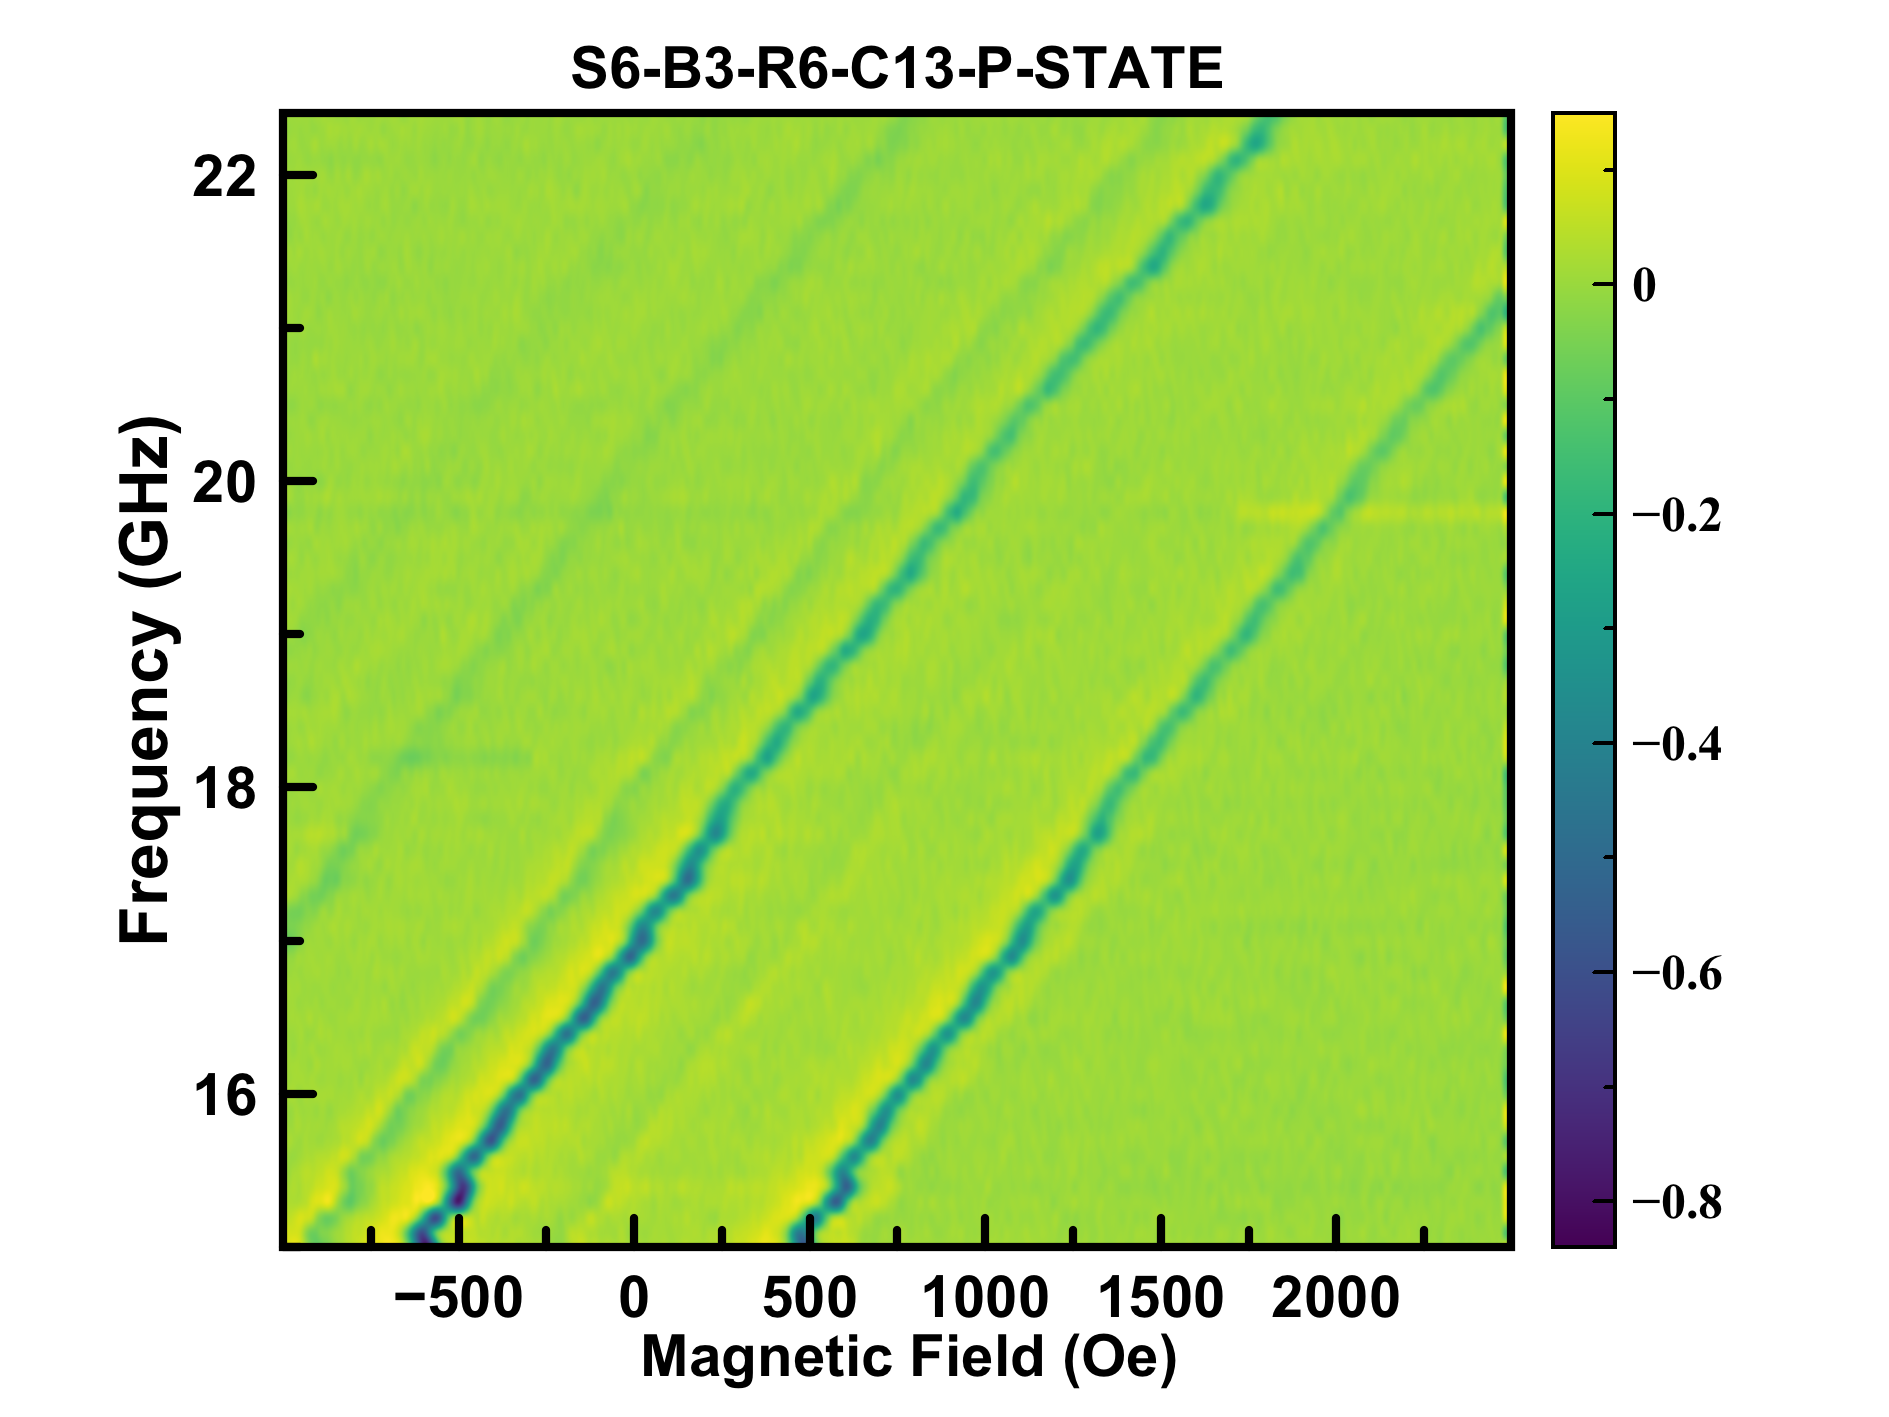
\includegraphics[width=75mm]{fig/in-plane/S6-B3-R6-C13-P-STATE}}
\caption{2D contour plot of ST-FMR spectrum taken at AP state(left) and P state(right). Both AP and P state has four lowest obvious spin-wave modes but with different mode spacings.}
\end{figure}

When we have a big MTJ device and the density of spin-wave modes is large due to later confinement, it is more difficult to identify all the modes excited in the spectrum. Fig.\ref{fig:S6AP} shows a ST-FMR 2D contour plot of a $120*60  nm^2$ device. At least we can identify four obvious spin-wave modes from this spectrum with lowest two modes very close to each other. If we focus on one constant-field vertical line, we can see the first mode and the second mode are very close to each other while the amplitude of the first mode is much smaller than the second one. If we look at the 2D ST-FMR contour plot at the parallel state shown in the Fig.\ref{fig:S6P}, it would not make the spin-wave modes identification easier. At the parallel state we also have identified four spin-wave modes with a decent larger gap between the first mode and the second. However we know that the mode spacings are determined by the exchange stiffness of the free layer and there should not be such a obvious difference between the AP and P state. There are generally(which is not necessarily present in the current case) two problems when measuring the MTJ at the parallel state. First of all, the ST-FMR signal is proportional to the absolute value of resistance oscillations under the ac current drive, which is less dominant in the parallel state. This means the parallel state has less signal amplitude compared with the AP state, especially for the quasi-uniform mode. Another problem is that, at the parallel state, since the SAF top layer is parallel to the free layer, it might be possible to excite the SAF modes close to the free layer mode.


\begin{figure}[!ht]
\centering
\subfigure{\label{fig:S6APDC}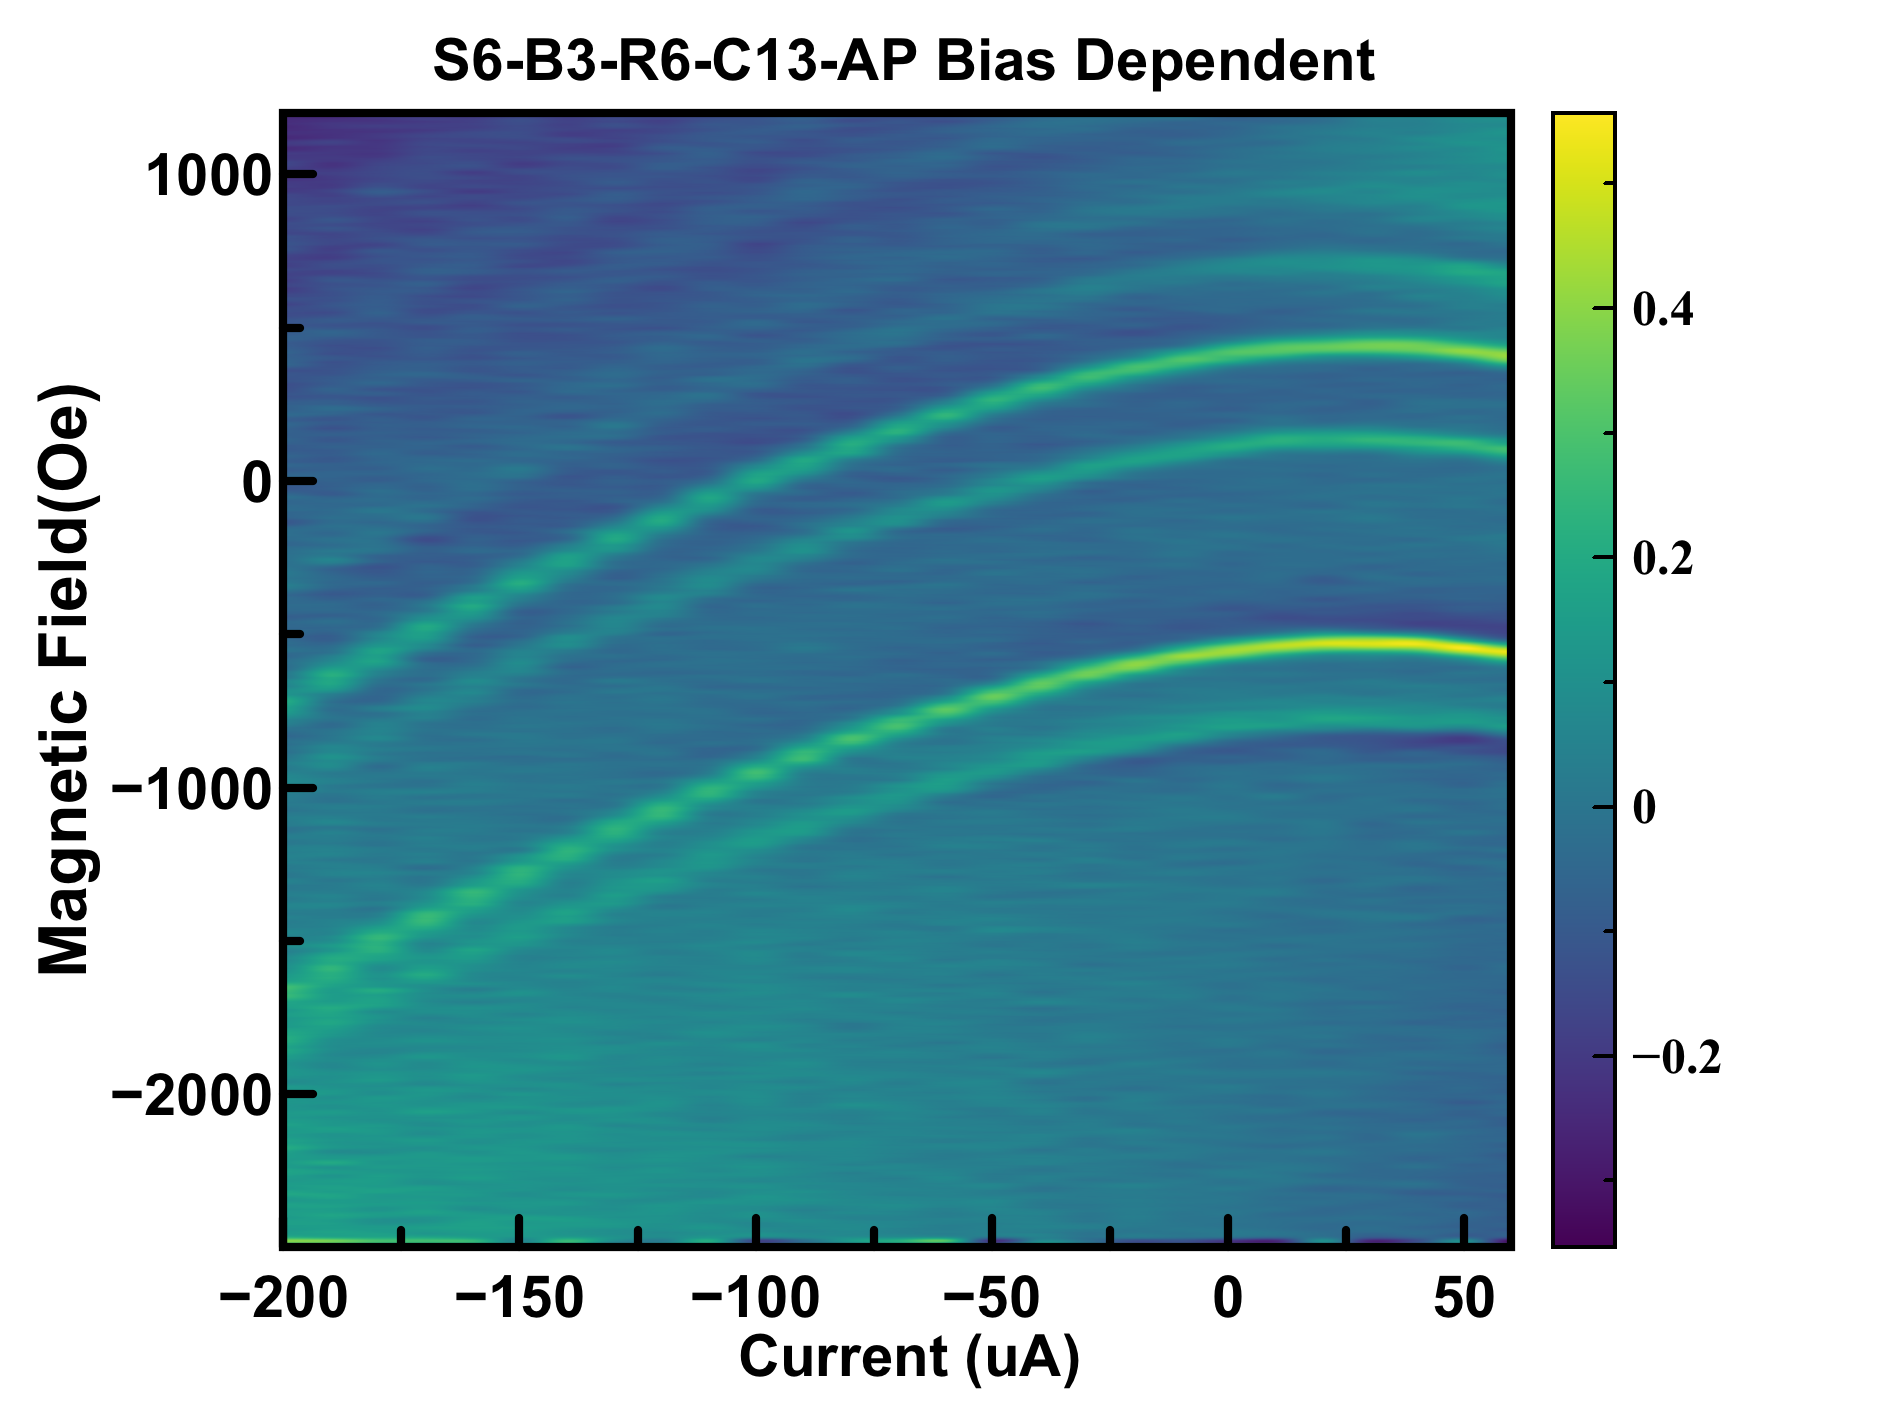
\includegraphics[width=75mm]{fig/in-plane/ap-dc}}
\subfigure{\label{fig:S6PDC}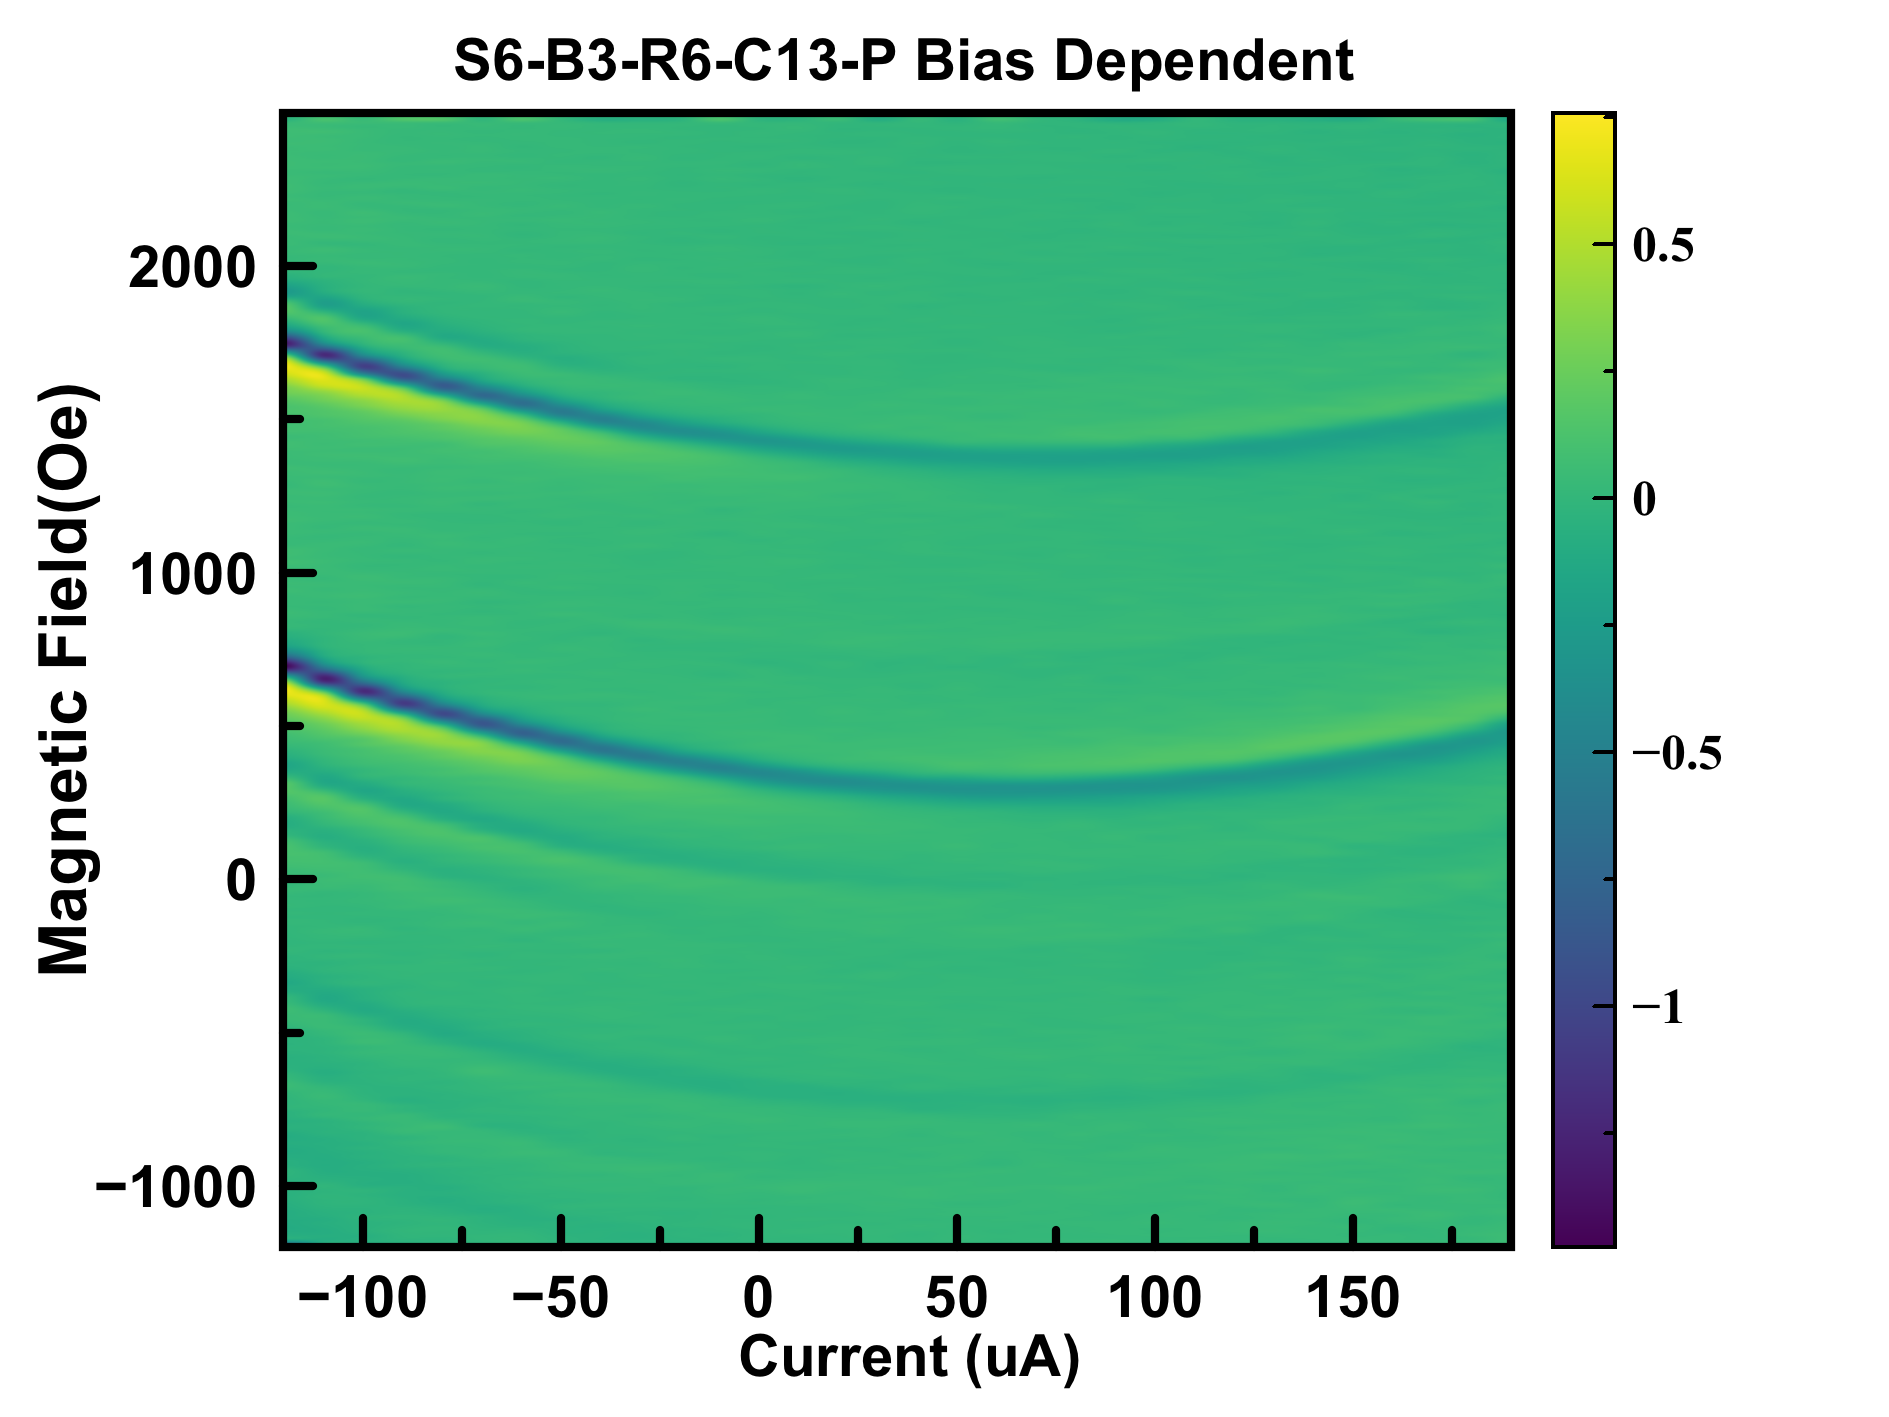
\includegraphics[width=75mm]{fig/in-plane/p-dc}}
\caption{Bias dependent ST-FMR spectrum taken at the constant driven frequency 16 GHz for both AP state(left) and P state(right). All the spin-wave modes have the same curvature versus bias.}
\end{figure}

The first type of measurements we can make to ensure we excite the free layer spin-wave modes only is to perform DC bias-dependent ST-FMR for both AP and P state. Because of the different spin torque polarity, the free layer and the SAF layer modes should have different curvature when applying the non-zero finite bias current. As we discussed in the previous section, the study of the linewidth as a function of dc bias can also be utilized to fit for the critical voltage of the MTJs. In Fig.\ref{fig:S6APDC} and Fig.\ref{fig:S6PDC} we have the bias dependent ST-FMR scan at the fix frequency 16 GHz for both AP and P state. What we find is that all the modes we observed at the previous ST-FMR 2D field dispersion contour plot have shown the same curvature under finite bias. This curvature is often determined by the combination of the voltage-controlled magnetic anisotropy and ohmic heating effect.


\begin{figure}[!ht]
\centering
\subfigure{\label{fig:S6APOUT}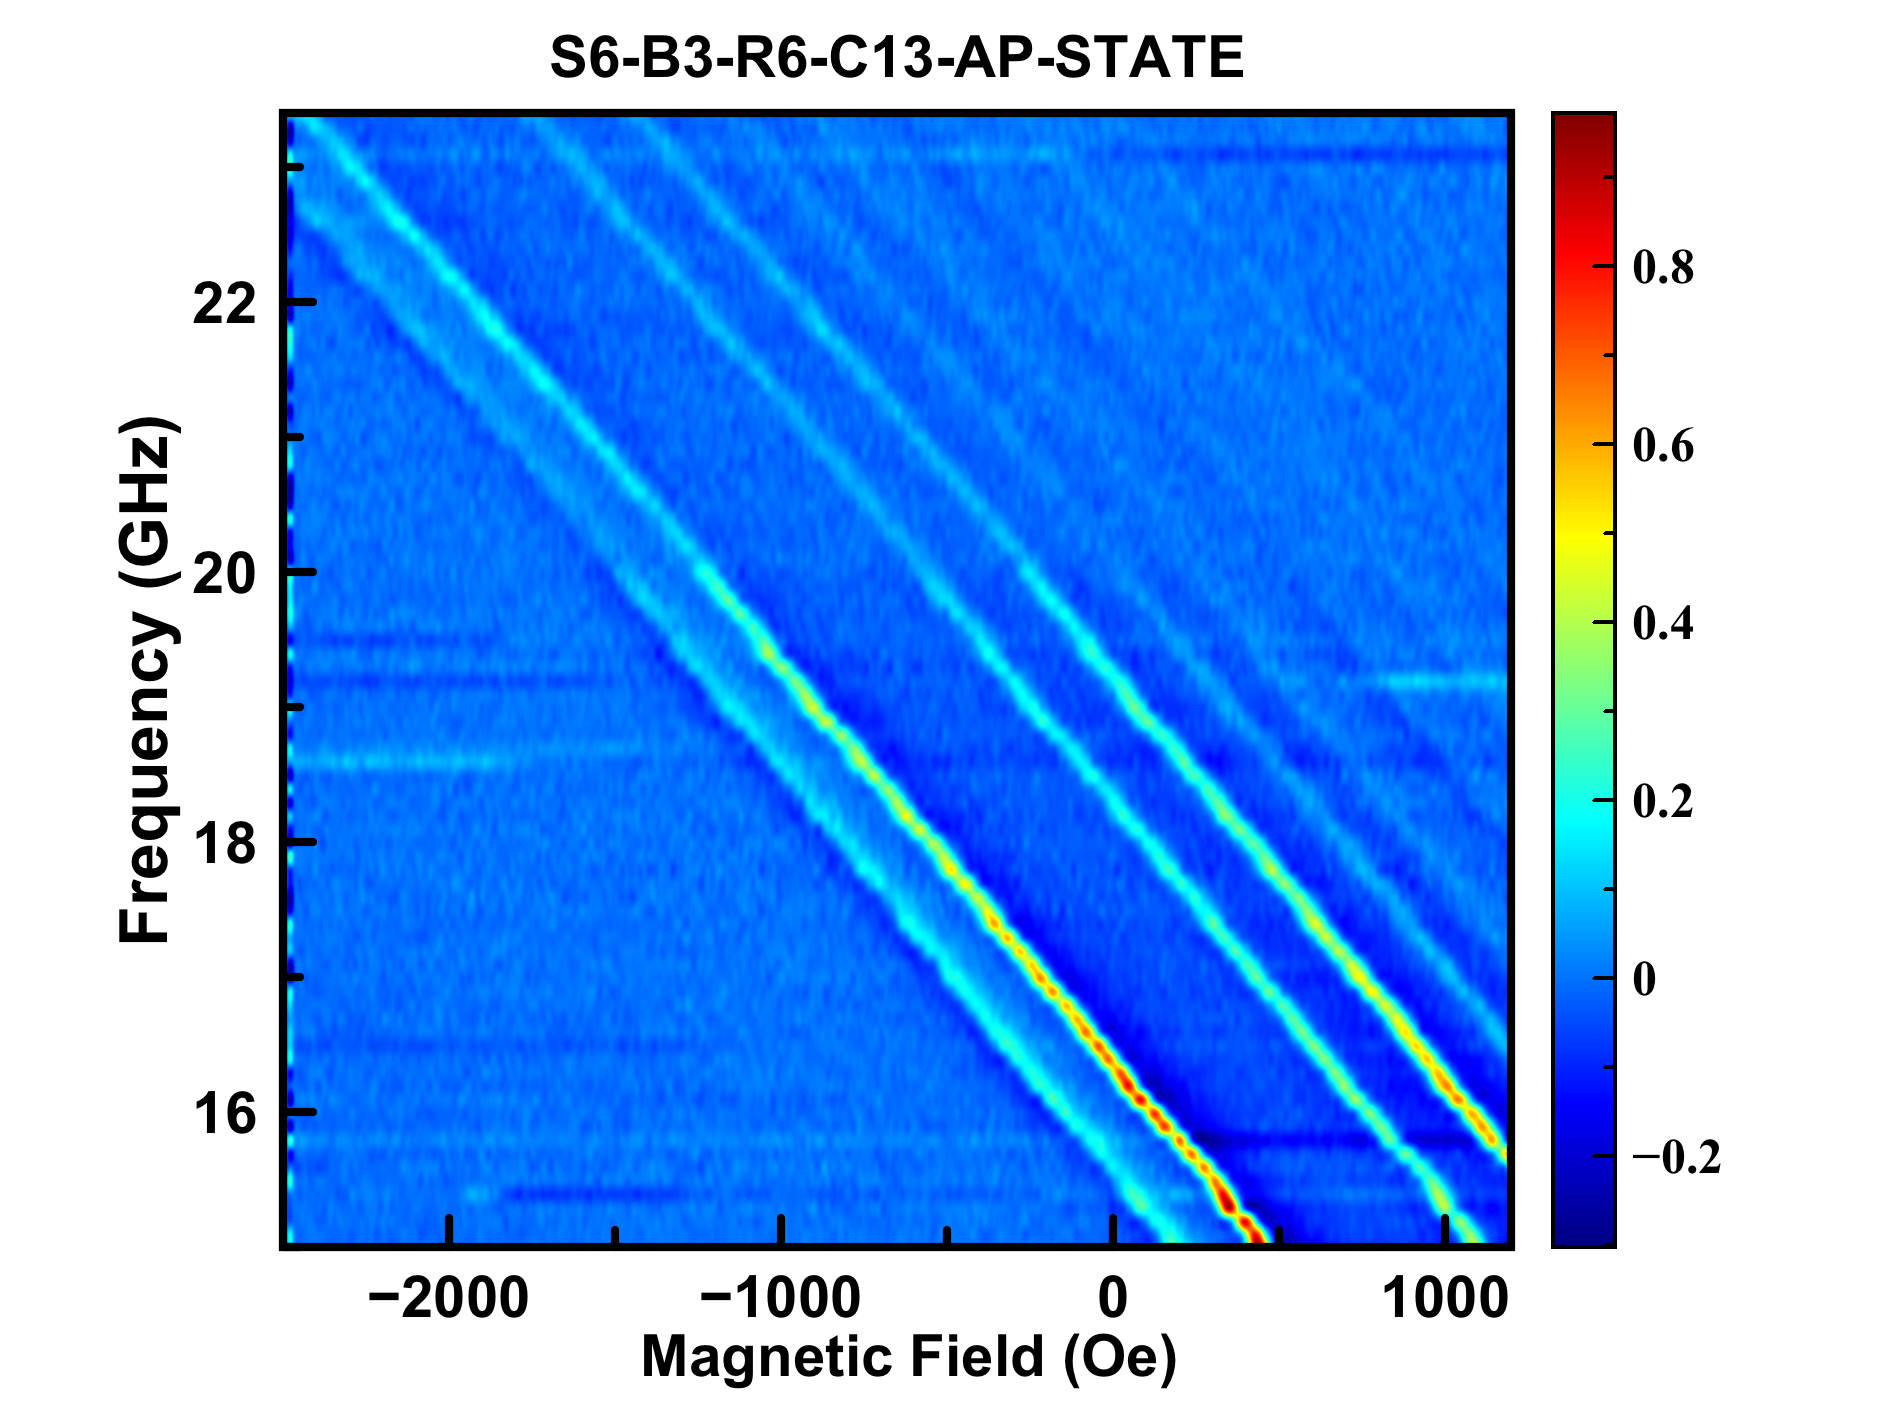
\includegraphics[width=75mm]{fig/in-plane/S6-B3-R6-C13-AP-STATE}}
\subfigure{\label{fig:S6APIN}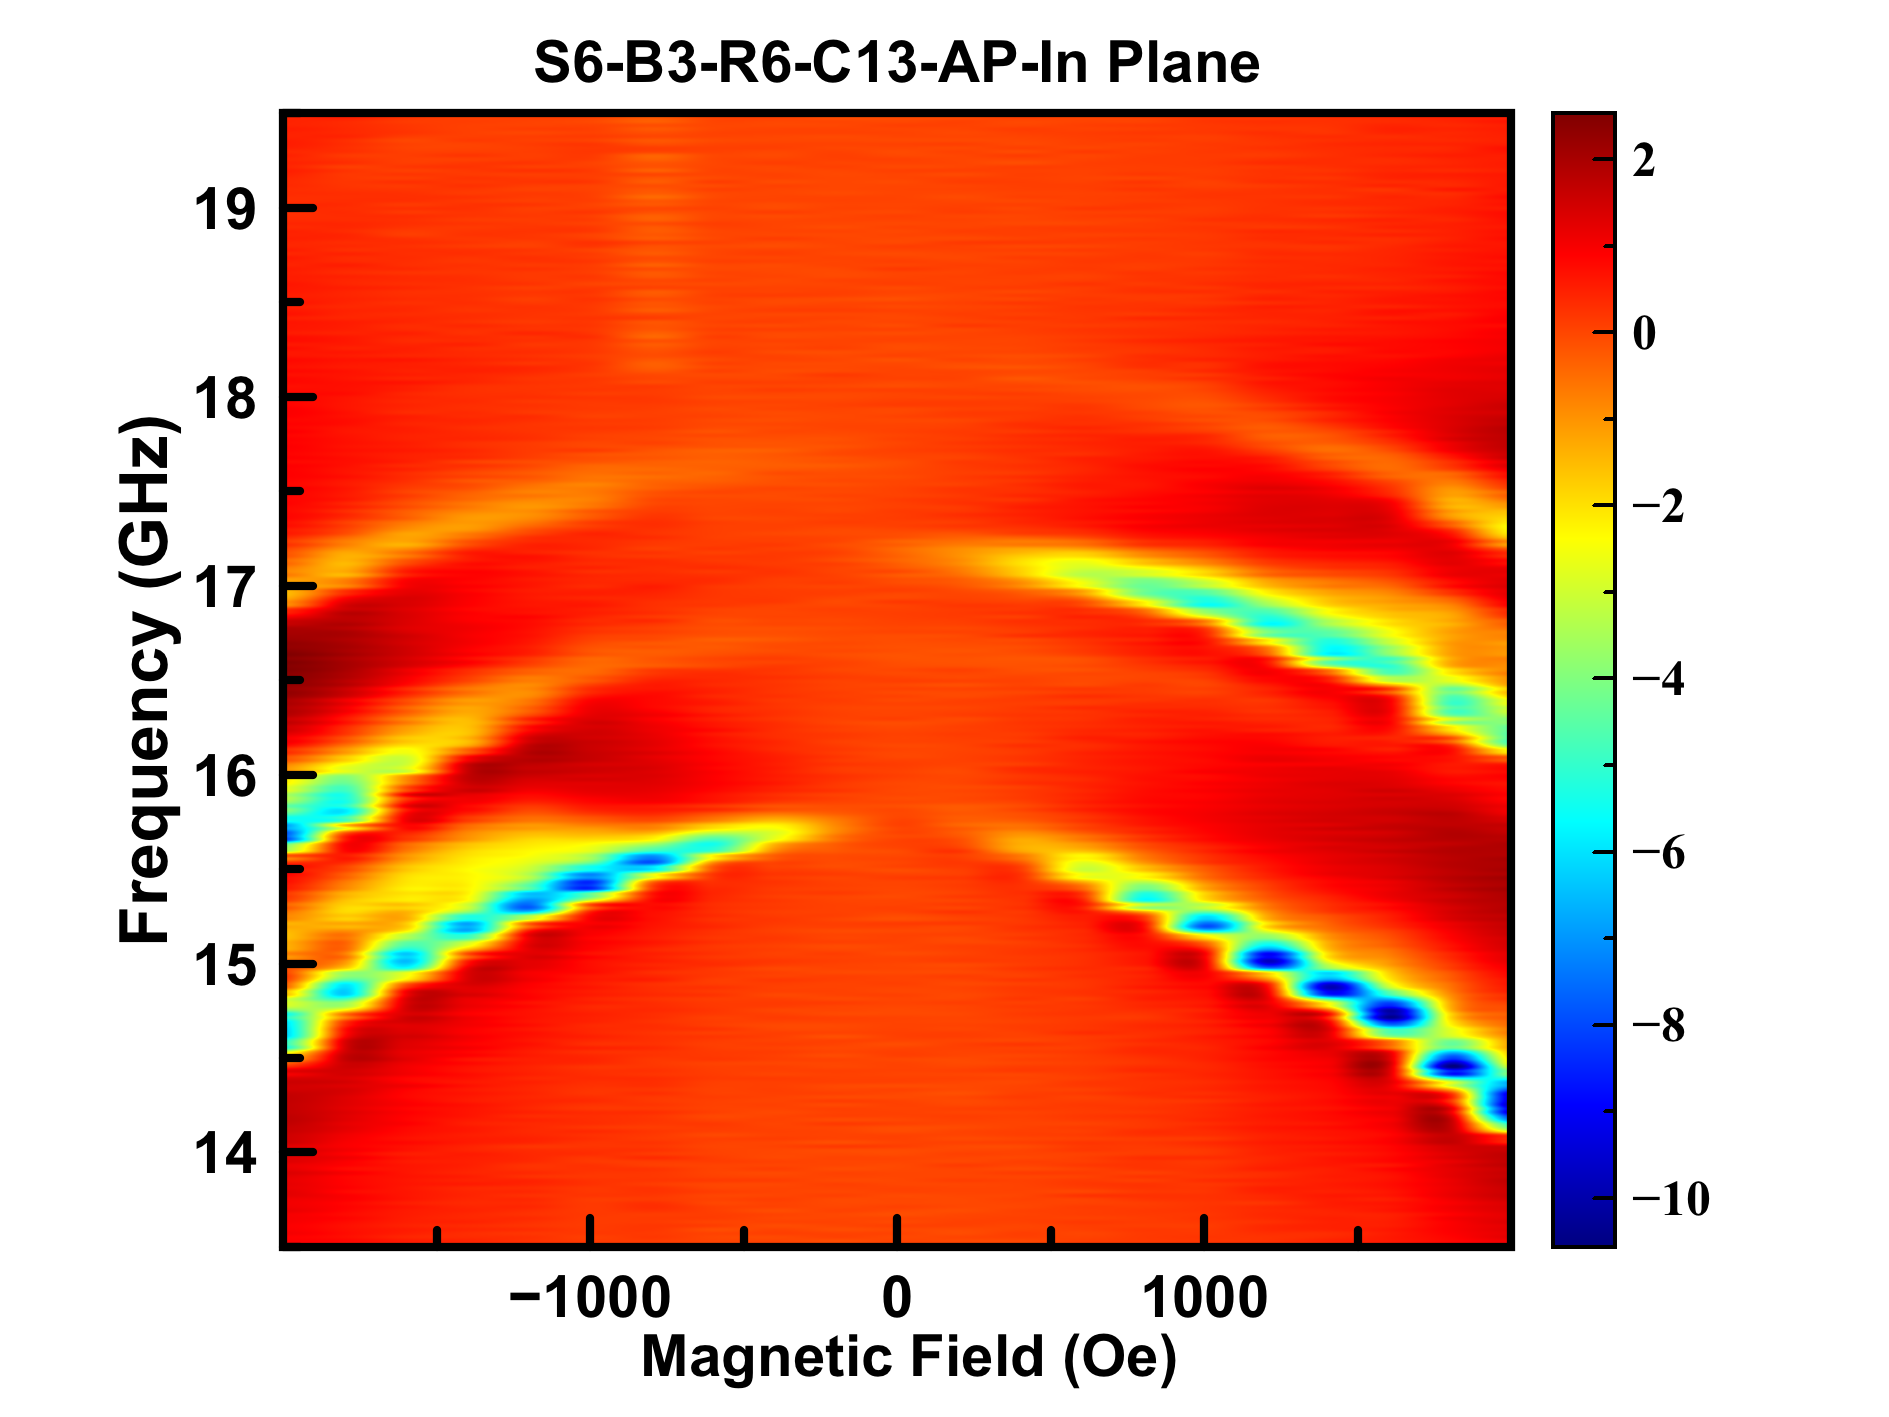
\includegraphics[width=75mm]{fig/in-plane/S6-B3-R6-C13-inplane}}
\caption{2D contour plot of ST-FMR spectrum taken at AP state with out-of-plane field applied(left) and in-plane field(right). Both spectrum has four lowest spin-wave modes with different relative amplitude.}
\end{figure}

So far we can conclude that all the spin-wave modes we saw in the out-of-plane ST-FMR measurements are from the free layer. Now we need to identify all the modes without missing some of the modes. We then perform ST-FMR measurement applying the in-plane magnetic field. When we apply the in-plane magnetic field to this MTJ with perpendicular magnetic anisotropy, we will create misalignment between the free layer and the fixed layer by introducing the hard axis magnetic field. From the Fig.\ref{fig:S6APIN} we see such a 2D spectrum with in-plane magnetic field applied at the AP state. In this measurement, the quasi-uniform mode has the largest amplitude compared with other modes due to introduced misalignment. It is also clear that the amplitude of the quasi-uniform mode decrease as the magnetic field decrease. When approaching zero magnetic field, the uniform mode almost becomes invisible. This also help us understand why under perpendicular magnetic field, the main mode is hard to excite. In the next step, we can fit for the modes we excited in the in-plane spectrum and compare with the out-of-plane data. Here for better comparison, we also show the out-of-plane spectrum for the AP state in the Fig.\ref{fig:S6APOUT}. From both the spectrum we can at lease identify four spin-wave modes and we can fit four of them at zero magnetic field(out-of-plane or in-plane). 


\begin{table}[h!]
\centering
\begin{tabular}{||c c c||} 
 \hline
 Experiment & Out-of-Plane & In-Plane\\ [0.5ex] 
 \hline\hline
 Mode 0 (GHz) & 15.63 & 15.42\\ 
 \hline
 Mode 1 (GHz) & 16.33 & 16.23\\
 \hline
 Mode 2 (GHz) & 18.28 & 18.28\\
 \hline
 Mode 3 (GHz) & 19.22 & 19.12 \\ [1ex] 
 \hline
\end{tabular}
\caption{Comparisons between four lowest spin-wave modes at AP state at zero magnetic field with different magnetic field direction(easy-axis out-of-plane and hard-axis in-plane) applied.}
\label{table:APtoP}
\end{table}

The table \ref{table:APtoP} summarizes the mode fitting results. Within certain deviations, it can be seen from the above results that we have good agreements between out-of-plane and in-plane measurements. Moreover, since in-plane hard-axis measurements are able to excite all the spin-wave modes, we can now be confident about our out-of-plane measurement without missing the free layer modes.

